\begin{flushright} {\tiny {\color{gray} pair\_p2p1p0.tex}} \end{flushright}
%~~~~~~~~~~~~~~~~~~~~~~~~~~~~~~~~~~~~~~~~~~~~~~~~~~~~~~~~~~~~~~~~~~~~~~~~~~~~~~~~~~~~~~~~~~~~~~~~~~

This element pair is discussed in 5.3.3 of Elman, Silvester and Wathen: 

``[Another] possibility is to construct a hybrid pressure approximation by 
combining the continuous linear pressure approximation with the discontinuous constant pres-
sure approximation. The resulting mixed method is referred to as the $P_2-P_{-1*}$ 
approximation and enjoys the best of both worlds; it has locally 
incompressibility, and yet it does not have its accuracy compromised by
the lower order pressure [of $P_2\times P_0$]. 
Perhaps surprisingly, this element is also uniformly stable.'' 

\begin{center}
\includegraphics[width=7cm]{images/pair_p2p1p0/elsw}\\
{\captionfont Taken from \textcite{elsw}.}
\end{center}

In Gresho \& Sani table 3.13-1: ``LBB stable yes. Better than P2P1, element mass balance.
more work than P2P1. 2 hydrostatic modes. Second order.'' 

\begin{center}
\includegraphics[width=4cm]{images/pair_p2p1p0/grsa2}
\includegraphics[width=12cm]{images/pair_p2p1p0/grsa1}\\
{\captionfont Taken from \textcite{grsa}. Unfortunately they do not provide a source for 
its origin, for the LBB-stability proof, or any source at all, actually.}
\end{center}

Looking at the figure above, it is clear that the $P_1$ space is to be understood 
as a continuous pressure space, with an additional constant bubble. 

For the continuous $P_1$ space, we have the following reference element
\begin{center}
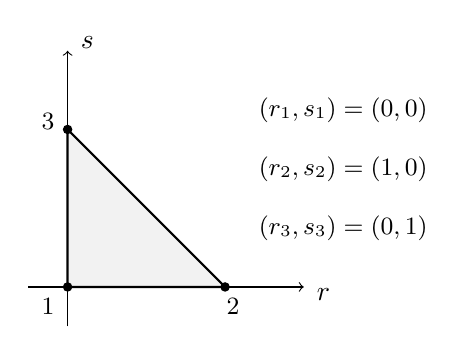
\begin{tikzpicture}
\draw[fill=gray!10,gray!10] (0.5,0.5)--(2.5,0.5)--(0.5,2.5)--cycle;
\draw[thick] (0.5,0.5)--(2.5,0.5)--(0.5,2.5)--cycle;
\draw [->] (0,0.5) -- (3.5,0.5);
\draw [->] (0.5,0) -- (0.5,3.5);
\node[] at (3.75,0.4) {$r$};
\node[] at (0.75,3.6) {$s$};
\draw[black,fill=black] (0.5,0.5)   circle (1.5pt);
\draw[black,fill=black] (2.5,0.5)   circle (1.5pt);
\draw[black,fill=black] (0.5,2.5)   circle (1.5pt);
\node[] at (0.25,0.25) {\small $1$};
\node[] at (2.6,0.25) {\small $2$};
\node[] at (0.25,2.6) {\small $3$};
\node[] at (4,2.75) {\small $(r_1,s_1)=(0,0)$};
\node[] at (4,2) {\small $(r_2,s_2)=(1,0)$};
\node[] at (4,1.25) {\small $(r_3,s_3)=(0,1)$};
\end{tikzpicture}
\end{center}
and the basis functions are simply
\begin{eqnarray}
\bN_1(r,s) &=& 1-r-s \\
\bN_2(r,s) &=& r \\
\bN_3(r,s) &=& s 
\end{eqnarray}
with the interpolation requirement $\bN_i(r_j,s_j)=\delta_{ij}$ fulfilled, as well as $\sum_i \bN_i=1$. 

Now, following the figure by Gresho and Sani, I build the reference element for the $P_1+P_0$ space:
\begin{center}
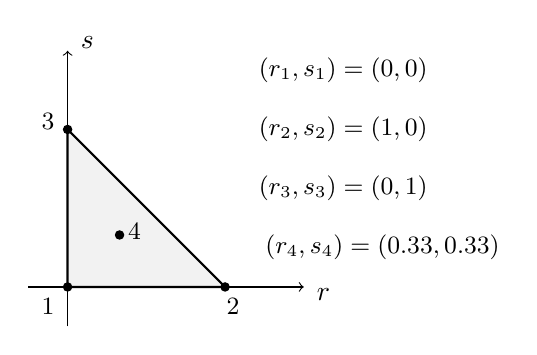
\begin{tikzpicture}
\draw[fill=gray!10,gray!10] (0.5,0.5)--(2.5,0.5)--(0.5,2.5)--cycle;
\draw[thick] (0.5,0.5)--(2.5,0.5)--(0.5,2.5)--cycle;
\draw [->] (0,0.5) -- (3.5,0.5);
\draw [->] (0.5,0) -- (0.5,3.5);
\node[] at (3.75,0.4) {$r$};
\node[] at (0.75,3.6) {$s$};
\draw[black,fill=black] (0.5,0.5)   circle (1.5pt);
\draw[black,fill=black] (2.5,0.5)   circle (1.5pt);
\draw[black,fill=black] (0.5,2.5)   circle (1.5pt);
\draw[black,fill=black] (1.16,1.16) circle (1.5pt);
\node[] at (0.25,0.25) {\small $1$};
\node[] at (2.6,0.25) {\small $2$};
\node[] at (0.25,2.6) {\small $3$};
\node[] at (1.35,1.2) {\small $4$};
\node[] at (4,3.25) {\small $(r_1,s_1)=(0,0)$};
\node[] at (4,2.5)    {\small $(r_2,s_2)=(1,0)$};
\node[] at (4,1.75) {\small $(r_3,s_3)=(0,1)$};
\node[] at (4.5,1) {\small $(r_4,s_4)=(0.33,0.33)$};
\end{tikzpicture}
\end{center}

$P_1+P_0$ means that the pressure inside the element is given by
\[
p^h(r,s) = a \bN_1(r,s)+ b\bN_2(r,s) + c\bN_3(r,s) + d\bN_4(r,s) 
\]
Note that it is then impossible to find $a,b,c,d$ such that the interpolation 
requirement $\bN_i(r_j,s_j)=\delta_{ij}$ is fulfilled.
In other words, the element is not interpolatory, i.e., there is no $\delta_{ij}$ property.% W.B. email

With regards to the 'element mass balance', W.B. states : 
``the mass conservation requires that the function that is constant 1 
on one cell and zero on all other cells is part of the function space. 
That is indeed true -- it's the $\bN_4$ function. Indeed, that's the purpose of 
the enrichment with the $P_0$ part. It is not necessary that {\it all} shape functions are discontinuous.''





\textcite{bocg12} (2012) state: ``[...] the pressure space $Q_h$ is defined as the sum of two finite 
element spaces, namely $P_k+P_0$ ($k \ge d- 1$) [...]for the enhanced Hood–Taylor [...]. 
However, it can be easily observed that the sum is not direct, 
since globally constant functions can be represented exactly by means of piecewise 
$P_0$ or continuous $P_k$ ($k \ge 1$) elements.
Concerning the implementation of the method, we avoid the computation of the basis
functions of such a finite element by testing the discrete problem (2.3) with the basis 
functions of the two subspaces separately. By the above discussion it turns out that the resulting
matrix is rank-deficient, with kernel of dimension 1.''



